\documentclass[a4paper,12pt]{article}
\usepackage{../../mypackages}
\usepackage{../../macros}

\setlength{\parindent}{0pt}


\begin{document}

\title{Chapitre 4 : L'atome / Les molécules}
\author{N. Bancel}
\date{Octobre 2024}
\maketitle

\section{Exercice 1}

\begin{figure}[H]
  \centering
  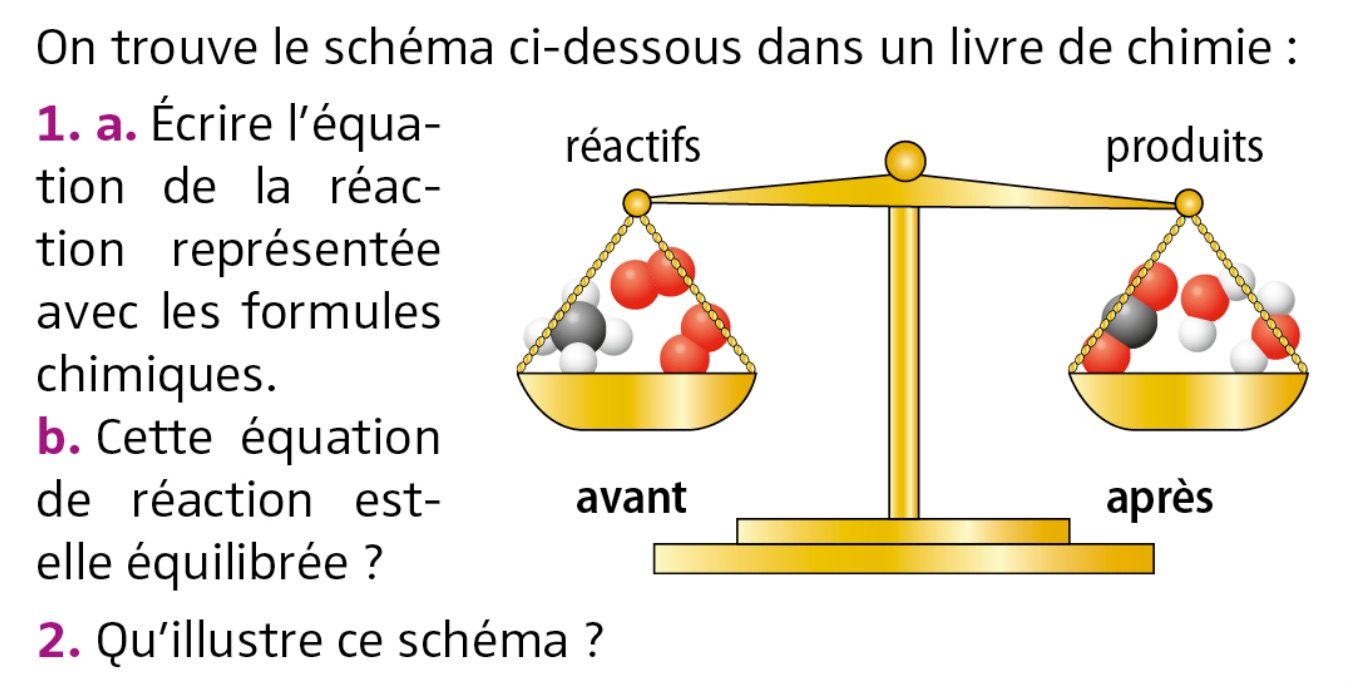
\includegraphics[width=0.8\linewidth]{04_02_01.jpg}
  \caption{\label{} Exercice 4}
\end{figure}

\section{Exercice 2}

\begin{figure}[H]
  \centering
  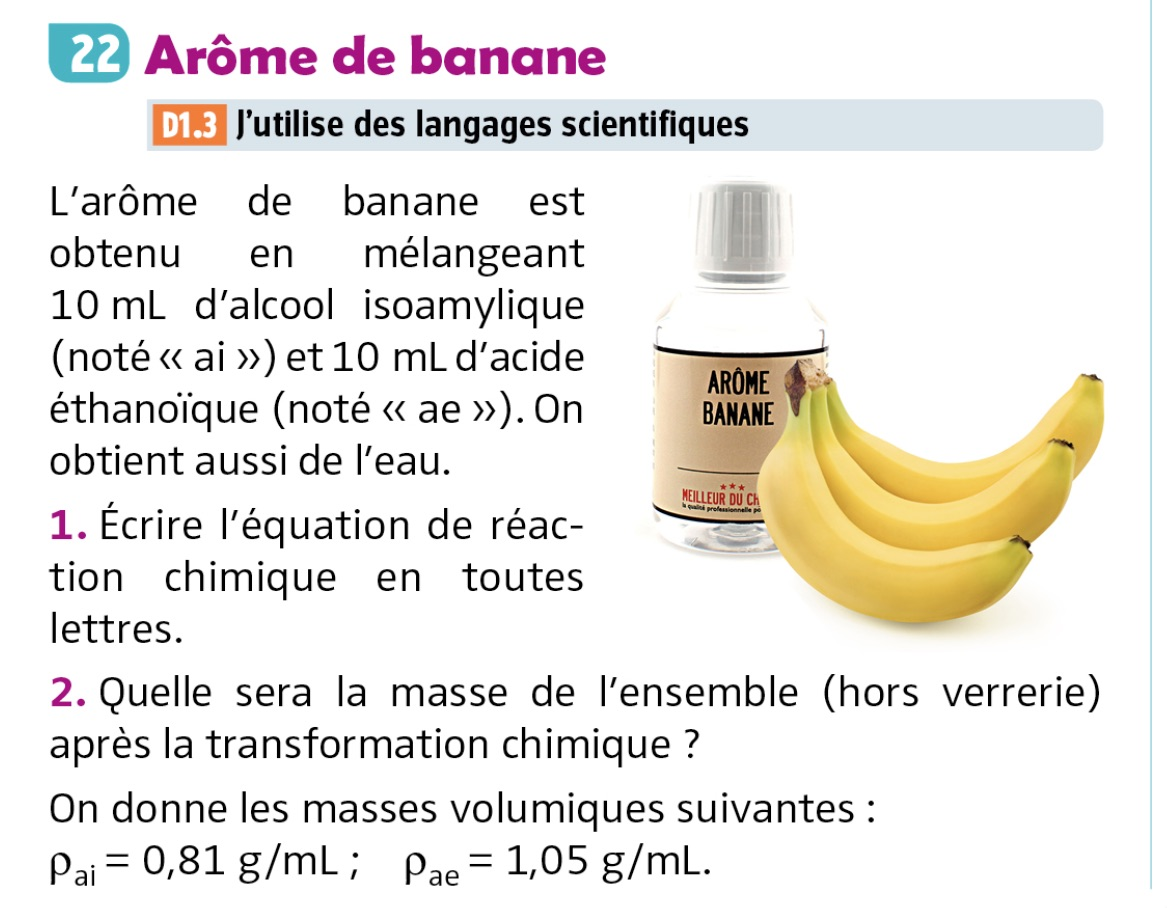
\includegraphics[width=0.8\linewidth]{04_02_02.jpg}
  \caption{\label{} Exercice 5}
\end{figure}

\section{Exercice 3}

\begin{itemize}[noitemsep]
\item Dans chaque réaction ci-dessous, essaie de nommer et identifier les espèces chimiques connues 
\item Identifie les réactifs, et les produits
\item Equilibre l'équation de réaction suivantes
\end{itemize} 

\begin{enumerate}
  \item \ce{C3H8 + O2 -> CO2 + H2O}
  \item \ce{H2O + O2 -> H2O2}
  \item \ce{CH4 + O2 -> CO2 + H2O}
  \item \ce{H2O -> H2 + O2}
  \item \ce{N2 + H2 -> NH3}
  \item \ce{C2H6 + O2 -> CO2 + H2O}
  \item \ce{C + O2 -> CO}
  \item \ce{CH4O + O2 -> CO2 + H2O}
  \item \ce{Fe3O4 + H2 -> Fe + H2O}
\end{enumerate} 

\section{Exercice 4}

\begin{figure}[H]
  \centering
  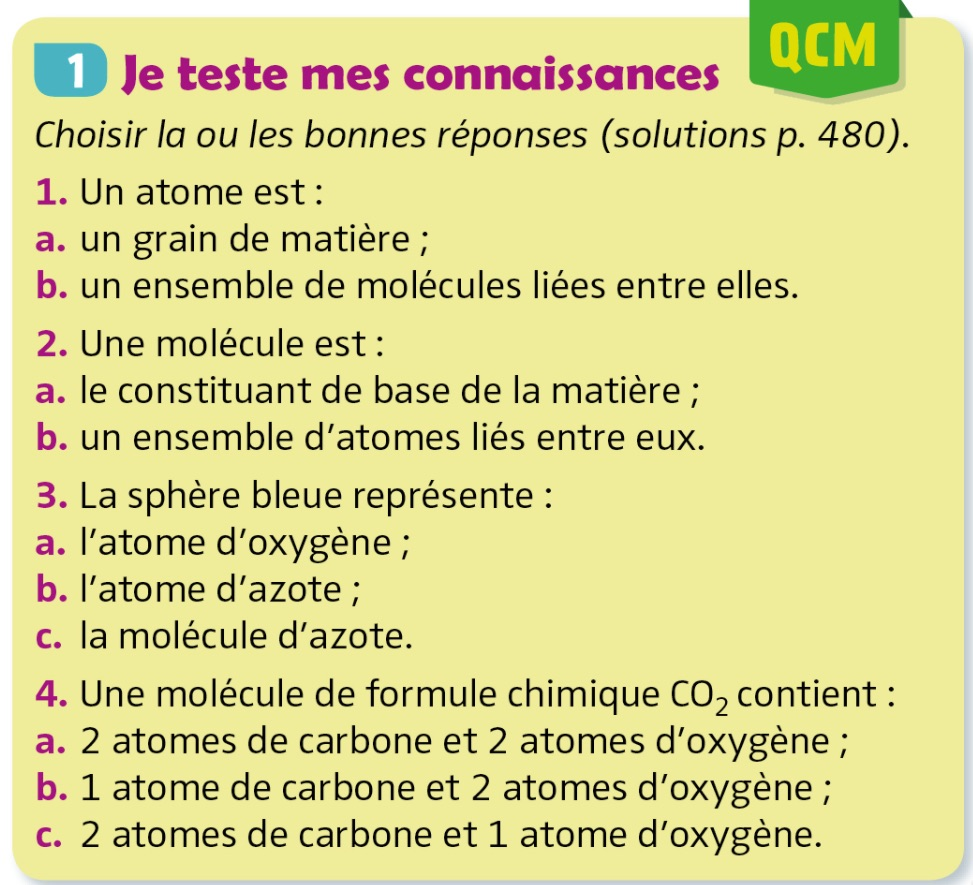
\includegraphics[width=0.9\linewidth]{04_02_03.jpg}
  \caption{\label{} Exercice 1}
\end{figure}

\section{Exercice 5}

\begin{figure}[H]
  \centering
  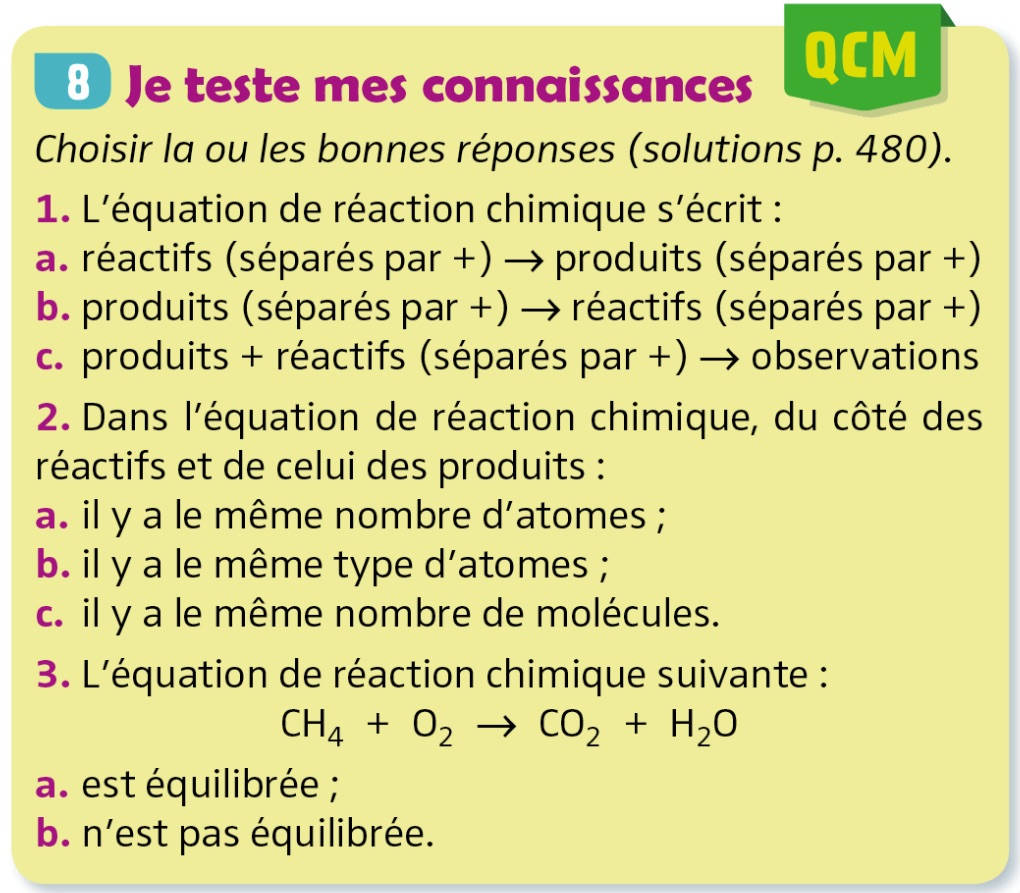
\includegraphics[width=0.9\linewidth]{04_02_04.jpg}
  \caption{\label{} Exercice 2}
\end{figure}

\section{Exercice 6}

\begin{figure}[H]
  \centering
  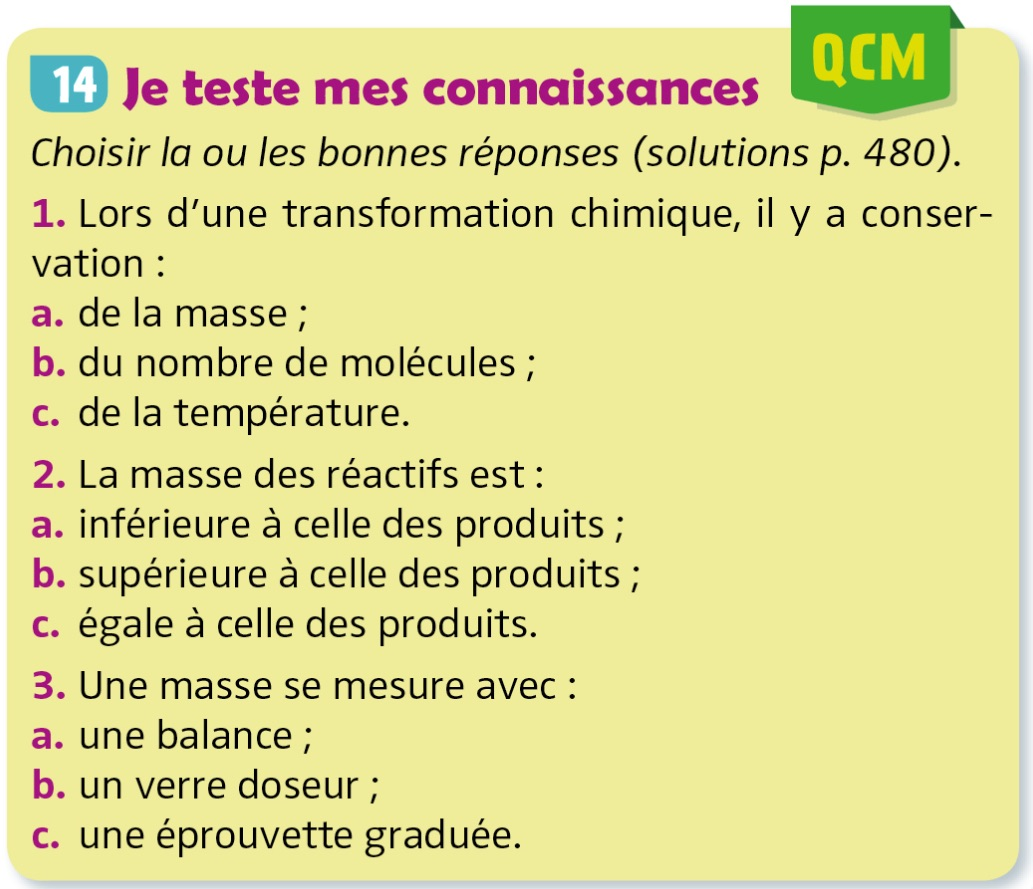
\includegraphics[width=0.9\linewidth]{04_02_05.jpg}
  \caption{\label{} Exercice 3}
\end{figure}

\end{document}
